\section{Introduction}
\subsection{Robots in factories}


\begin{frame}{Industry 4.0: Logistic enhanced by robotics}
    \centering

    Improve flexibility and efficiency of factories using a fleet of Autonomous Mobile Robots (AMRs).

    ~~

\begin{columns}
    \begin{column}{0.6\textwidth}
        \pause
        High-level robotic agent to:
        \begin{itemize}
            \pause
            \item Automate task allocation to AMR
            \pause
            \item Deal with contingencies and deadlines
            \pause
            \item Optimize the overall process in function of time, energy, etc.
        \end{itemize}
    \end{column}
    \begin{column}{0.4\textwidth}
        \onslide<1->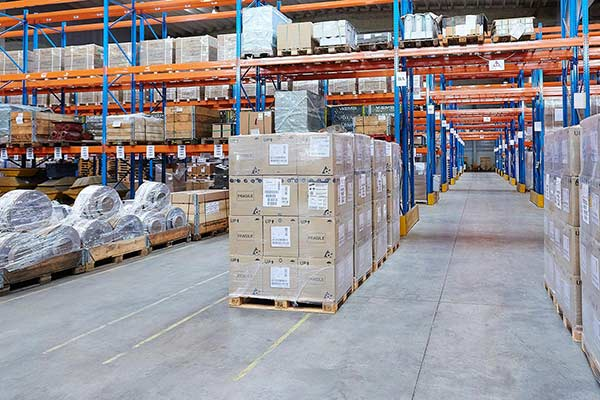
\includegraphics[width = \textwidth]{images/logisticsolutions.jpg}
    \end{column}
\end{columns}
\end{frame}

\begin{frame}{Running example : factory simulator with an emphasis on deliberation}
    \begin{columns}
        \begin{column}{0.5\textwidth}
            2D factory simulator to study scheduling and resource allocation strategies.
        \end{column}
        \begin{column}{0.4\textwidth}
            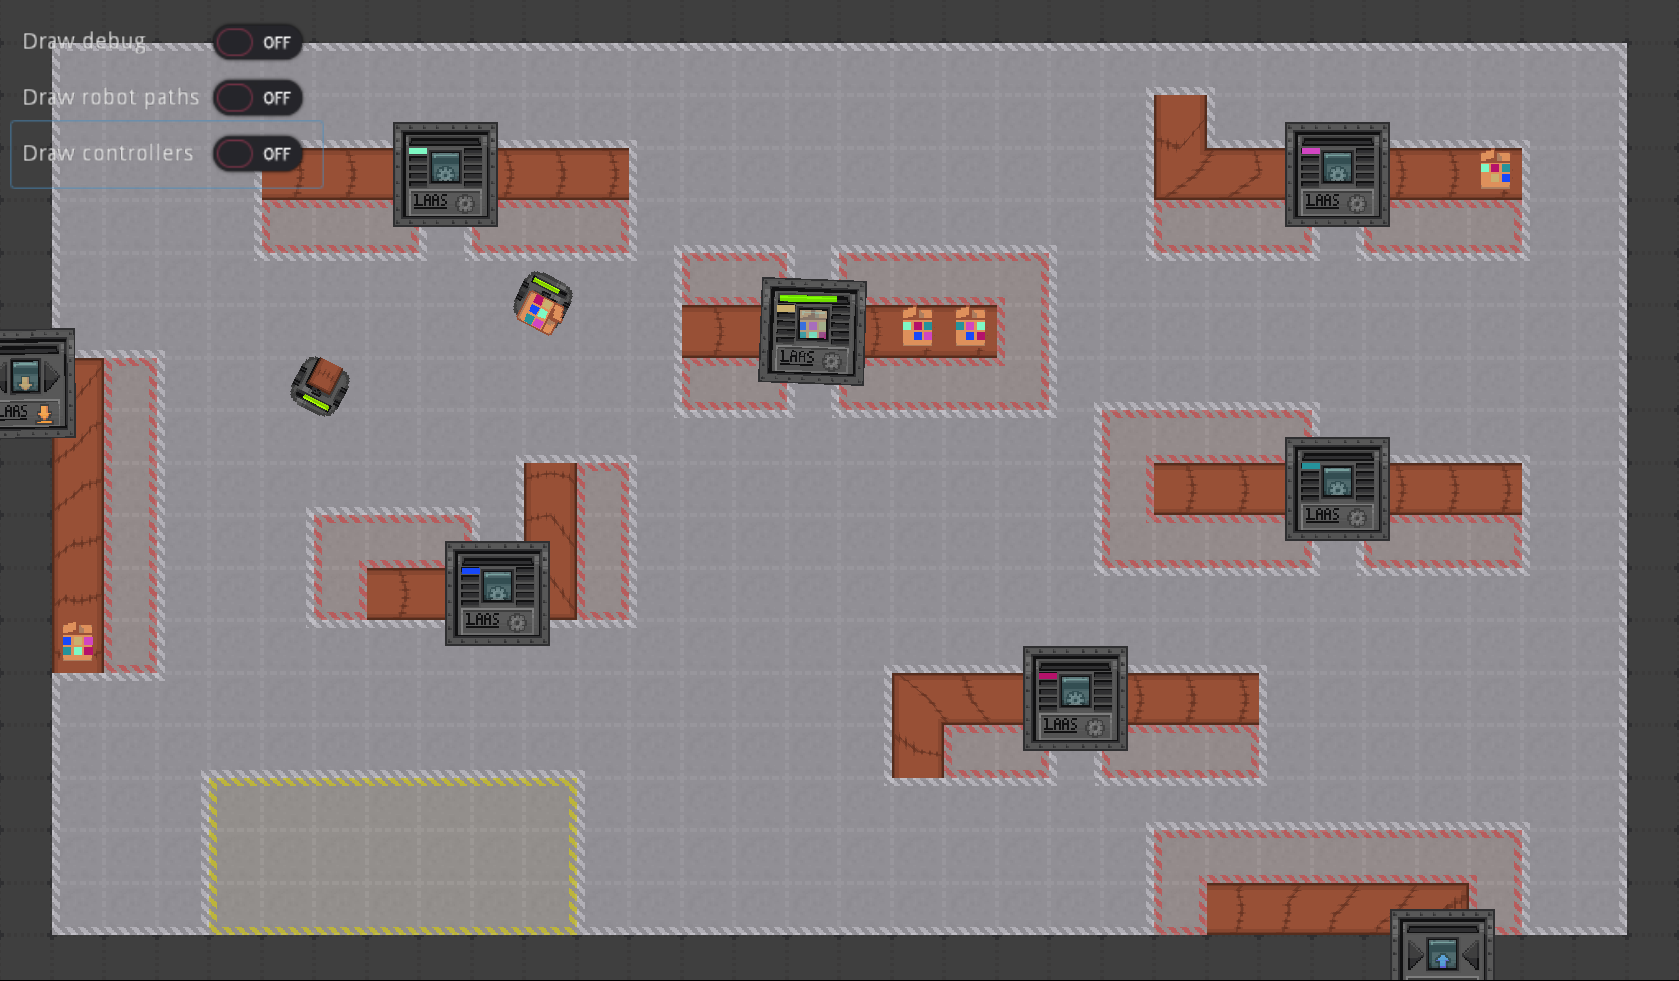
\includegraphics[width=\linewidth]{images/gobot-rae.png}
        \end{column}
    \end{columns}
    
    ~~

\pause
    \centering
    \emph{Environment}

~~

\pause
    \begin{columns}
        \begin{column}{0.3\textwidth}
            \centering
            Package

            ~~

            
\includegraphics[width = 0.5\textwidth]{images/godot/package.png}
        \end{column}
        \pause
        \begin{column}{0.3\textwidth}
            \centering
            Machine

            ~~

            
\includegraphics[width = 0.5\textwidth]{images/godot/machine_texture.png}

        \end{column}
        \pause
        \begin{column}{0.3\textwidth}
            \centering
            Robot

            ~~

            
\includegraphics[width = 0.5\textwidth]{images/godot/robot_texture.png}
        \end{column}
    \end{columns}

    % \begin{columns}
    %     \begin{column}{0.2\textwidth}
            
    %     \end{column}
    %     \begin{column}{0.7\textwidth}
    %         Machines
    %         \begin{itemize}
    %             \item Processing : does a predefined list of process for packages
    %             \item Input: generate packages
    %             \item Output: gather fully processed packages
    %         \end{itemize}
    %     \end{column}
    % \end{columns}

    % ~

    % \begin{columns}
    %     \begin{column}{0.2\textwidth}
            
    %     \end{column}
    %     \begin{column}{0.7\textwidth}
    %         Robots : manipulate packages
    %         \begin{itemize}
    %             \item commands: move, pick, place,\dots
    %             \item recharge at recharge areas
    %         \end{itemize}
    %     \end{column}
    % \end{columns}
\end{frame}

% \begin{frame}{Other logistic simulators}
%     \begin{columns}[t]
%         \begin{column}{0.5\textwidth}
%             \small
%             Robocup Logistic League Simulation \cite{niemuellerPlanningCompetitionLogistics2016}

%             \includegraphics[width = \linewidth]{images/robocup.png}
            
%         \end{column}
%         \begin{column}{0.5\textwidth}
%             \small
%             CraftBots \cite{nemiroDesigningAdaptableBenchmark2021}

%             \includegraphics[width = \linewidth]{images/craftbots.png}
%         \end{column}
%     \end{columns}
    
% \end{frame}

\begin{frame}{Mission of the robotic agent}
    \centering
Mission : Do all the processes of packages, and for each process of a package:
\begin{itemize}
    \pause
    \item Select a machine to do the process.
    \pause
    \item Select a robot to carry it to the machine.
\end{itemize}

\end{frame}

\subsection{Programming a robotic agent}

\begin{frame}{Programming the robotic agent in a hierarchical fashion}
    Define its behavior:
    \begin{itemize}
        \pause
        \item able to act in different contexts,
        \pause
        \item robust to hazards and errors,
        \pause
        \item reactive.
    \end{itemize}
    
    ~~
    
    Hierarchical representation of the agent skills.
    \begin{itemize}
        \pause
        \item Set of low-level capabilities: \textit{move, pick, place}
        \pause
        \item Set of high-level capabilities: \textit{process package}
        \pause
        \item Skills $\equiv$ different ways of achieving high-level capabilities
        \begin{itemize}
            \item operational model (executable)
            \item composition of lower-level capabilities
        \end{itemize}
        %\item Several levels of abstraction $\rightarrow$ ease deliberation.
    \end{itemize}
\end{frame}

\begin{frame}{Acting domain}
    \begin{columns}[T]
        \begin{column}{0.55\textwidth}
            Acting domain \textbf{$A_\Delta (A, T, M_t)$}
            \small
            \pause
            \begin{itemize}
             \item[$A$] : commands (low-level capabilities)
             \pause
             \item[$T$] : tasks (high-level capabilities)
             \pause
             \item[$M_t$] : methods (skills):
             \begin{itemize}
                \item pre-conditions
                \item body (executable program)
             \end{itemize}
             
         \end{itemize}
        \end{column}
        \pause
        \begin{column}{0.45\textwidth}
            \begin{tikzpicture}
                \node[draw, ellipse, ultra thick] (t) {\textit{take}} [sibling distance = 3.5cm]
                    child {node[draw, ultra thick] (m1) {$m_1$} edge from parent [dashed]
                    child {node[draw,rounded corners, ultra thick, solid] (a1) {$pick$} edge from parent
                    }} 
                    child {node[draw, ultra thick] (m2) {$m_2$} edge from parent [dashed] [sibling distance = 1.5cm]
                    child {node[draw, ellipse, ultra thick, solid] (a2) {$move$} edge from parent [solid]}
                    child {node[draw, rounded corners, solid, ultra thick] {$pick$} edge from parent [solid]}};
                \node[right = 0em of t] {$\in T$};
                \node[right = 0em of m1] {$\in M_t$};
                \node[right = 0em of m2] {$\in M_t$};
                \node[right = 0em of a1] {$\in A$};
    
            \end{tikzpicture}
    
        \end{column}
    \end{columns}
\end{frame}

\begin{frame}{Refinement Acting Engine (RAE): deliberation algorithms using hierarchical operational models}
    Features of the system:
    \begin{itemize}
        \pause
        \item Monitor task and command execution
        \pause
        \item Perform multiple tasks in parallel
          \pause
          \item \textbf{Automated} refinement of task into method and parameters choice 
      \end{itemize}
      \centering
      \begin{tikzpicture}
          \node[] (task) {$\tau(p_1,\dots,p_n)$};
          \node[below = 2em of task] (method) {$m(p_1,\dots,p_n, \dots, p_m)$};
          \path[->] (task) edge node[right, midway] {refinement} (method);
      \end{tikzpicture}
\end{frame}

\begin{frame}{RAE functioning}
    \begin{columns}[T]
  
        \begin{column}{0.65\textwidth}
            
            Algorithms:
            \small
            \begin{itemize}
                \setlength{\leftmargini}{-1pt}
                \onslide<2->
                \item \textbf{Main:} 
                \begin{itemize}
                    \item Receive $\tau$ (task or event);
                    
                    add it to the \textbf{agenda} (ongoing tasks)
                    \onslide<3->
                    \item Refine $\tau$: \textbf{Select} an applicable method $m$ for $\tau$
                    \onslide<4->
                    \item \textbf{Progress} $m$
                \end{itemize}
                \onslide<5->
                \item \textbf{Progress:}
                    \begin{itemize}
                        \onslide<6->
                        \item Monitor execution of $m$.
                        \onslide<7->
                        \item Refine subtasks in $m$.    
                        \onslide<8->
                        \item Monitor execution of subtasks.
                        \onslide<9->
                        \item \textbf{Retry} $\tau$ in case of \emph{failure}:
                    
                    Call \textbf{Select} to get a new method;
                    
                    \textbf{Progress} the new method.
                    \end{itemize}
            \end{itemize}
        \end{column}
        \begin{column}{0.35\textwidth}
            \begin{tikzpicture}
                \onslide<2>
                \node[draw,ellipse, ultra thick] (t) {$take$};
                \onslide<3-11>
                \node[draw,ellipse, ultra thick, color = orange] (t) {$take$};
                \onslide<12>
                \node[draw,ellipse, ultra thick, color = green] (t) {$take$};
                \onslide<3>
                \node[draw, ultra thick, below= 2em of t, xshift = -2em] (m1) {$m_1$};
                \node[draw, ultra thick, below= 2em of t, xshift = 2em] (m2) {$m_2$};
                \onslide<4->
                \node[draw, ultra thick, below= 2em of t, xshift = -2em, color = gray] (m1) {$m_1$};
                \onslide<4-11>
                \node[draw, ultra thick, below= 2em of t, xshift = 2em, color = orange] (m2) {$m_2$};
                \onslide<12>
                \node[draw, ultra thick, below= 2em of t, xshift = 2em, color = green] (m2) {$m_2$};
                \onslide<3->
                \path[-] (t) edge (m1) (t) edge (m2);
                \onslide<5-10>
                \node[draw,rounded corners, ultra thick, solid, below = 2em of m2, xshift = 2em] (a1) {$pick$};
                \onslide<11>
                \node[draw,rounded corners, ultra thick, solid, below = 2em of m2, xshift = 2em, color = orange] (a1) {$pick$};
                \onslide<12>
                \node[draw,rounded corners, ultra thick, solid, below = 2em of m2, xshift = 2em, color = green] (a1) {$pick$};
                \onslide<5>
                \node[draw,ellipse, ultra thick, solid, below = 2em of m2, xshift = -2em] (t2) {$move$};
                \onslide<6-9>
                \node[draw,ellipse, ultra thick, solid, below = 2em of m2, xshift = -2em, color = orange] (t2) {$move$};
                \onslide<10->
                \node[draw,ellipse, ultra thick, solid, below = 2em of m2, xshift = -2em, color = green] (t2) {$move$};
  
  
                \onslide<5->
                \path[-] (m2) edge (a1) (m2) edge(t2);
  
  
                \onslide<7>
                \node[draw, ultra thick, below = 2em of t2, xshift = -1.5em] (m3) {$m_3$};
                \node[draw, ultra thick, below = 2em of t2, xshift = 1.5em] (m4) {$m_4$};
                \path[-] (t2) edge  (m3) (t2) edge (m4);
                
                \onslide<8>
                \node[draw, ultra thick, below = 2em of t2, xshift = -1.5em, color = orange] (m3) {$m_3$};
                \node[draw, ultra thick, below = 2em of t2, xshift = 1.5em, color = gray] (m4) {$m_4$};
                \path[-] (t2) edge  (m3) (t2) edge (m4);

                \onslide<9>
                \node[draw, ultra thick, below = 2em of t2, xshift = 1.5em, color = orange] (m4) {$m_4$};
                \onslide<9->
                \node[draw, ultra thick, below = 2em of t2, xshift = -1.5em, color = red] (m3) {$m_3$};
                \path[-] (t2) edge  (m3) (t2) edge (m4);
                \onslide<10->
                \node[draw, ultra thick, below = 2em of t2, xshift = 1.5em, color = green] (m4) {$m_4$};
                
                \onslide<8->
                \node[below = 2em of m3, xshift = -1em] (e3) {};
                \node[below = 2em of m3, xshift = 1em] (e4) {};
                \path[-] (m3) edge  (e3) (m3) edge (e4);
  
                \onslide<8->
                \node[below = 2em of m4, xshift = -1em] (e5) {};
                \node[below = 2em of m4, xshift = 1em] (e6) {};
                \path[-] (m4) edge  (e5) (m4) edge (e6);
      
            \end{tikzpicture}
        \end{column}
    \end{columns}    
\end{frame}



\begin{frame}[fragile]{Simple scenario: one package}
    \centering
    \begin{columns}
        \begin{column}{0.5\textwidth}
            \centering
            
\includegraphics[width = 0.3\textwidth]{images/godot/package.png}
            
            \LARGE \emph{$\times 1$}
        \end{column}
        \begin{column}{0.5\textwidth}
            \centering
            
\includegraphics[width = 0.3\textwidth]{images/godot/robot_texture.png}
            
            \LARGE \emph{$\times 1$}
        \end{column}
    \end{columns}
    \pause
    \centering

    ~~

    Unique task \textit{process(?p)}

    Methods:
    
    \footnotesize
    \begin{columns}[t]
        \begin{column}{0.32\textwidth}
            \begin{align*}
                m1&(?p, ?r, ?m)\\
                pre: &\ proc(?p) \neq \emptyset \\
                 &battery(?r) > 40\% \\
                 &proc(?p)[1] \in proc(?m) \\
                 body:&take(?p,?r) \\
                     &carry(?p,?r,?m) \\
                     &process(?p)
            \end{align*}
        \end{column}
        \begin{column}{0.32\textwidth}
            \begin{align*}
                m2&(?p, ?r, ?m) \\
                pre: &\ proc(?p)  = \emptyset \\
                 &battery(?r) > 40\% \\
                 &kind(?m) = \text{output} \\
                 body:&take(?p,?r) \\
                     &carry(?p,?r,?m) \\
            \end{align*}
        \end{column}
        \begin{column}{0.32\textwidth}
            \begin{align*}
                m3&(?p, ?r) \\ 
                pre: &battery(?r) \leq 40\% \\
                 body:&recharge(?r) \\
                     &process(?p)
            \end{align*}
        \end{column}
    \end{columns}
    % \begin{align*}
    %     \text{task:} & \text{process(?p)}\\
    %     \text{methods:}& \\
    %     m1(?p, ?r, ?m) \\
    %     \text{pre:} & !empty(processes(?p)) \\
    %      &battery(?r) \leq 40\% \\
    %      &first(processes(?p)) \in processes(?m) \\
    %      body:&take(?p,?r) \\
    %          &carry(?p,?r,?m) \\
    %          &process(?p)
    % \end{align*}
    
\end{frame}

\begin{frame}{Running example with one package}
    \centering

    \includegraphics[width = 0.8\textwidth]{images/gobot-single-robot.png}
    
    \Large
    Video example: \href{https://youtu.be/Copcg6A6Cvo}{https://youtu.be/Copcg6A6Cvo}
\end{frame}

\subsection{Multi-agent problematics}

\begin{frame}{Several packages?}
    \begin{columns}
        \begin{column}{0.5\textwidth}
            \centering
            
\includegraphics[width = 0.5\textwidth]{images/godot/package.png}
            
            \Large $\times n$
        \end{column}
        \begin{column}{0.5\textwidth}
            \centering
            
\includegraphics[width = 0.5\textwidth]{images/godot/robot_texture.png}
            
            \LARGE $\times m$
        \end{column}
    \end{columns}
    
    ~
\pause
    New missions for the robotic agent:
    \begin{itemize}
        \pause
        \item Schedule package passage on machines
        \pause
        \item Allocate package displacement tasks to robots
        %\item Monitor the robots' batteries 
    \end{itemize}

    \centering
\end{frame}

\begin{frame}{Multi-agent refinement-based deliberation}
    RAE shortcomings:
    \begin{itemize}
        \pause
        \item Progression of tasks rely on Round Robin \pause$\rightarrow$ difficulty to interleave tasks using the same resources.
        \pause
        \item Methods limited to a sequence of actions
        %\item Difficulties to integrate sound planning from operational models due to implementation in Python.
    \end{itemize}

    ~~
    
\pause
    Solution: adapt RAE for multi-agents to
    \begin{itemize}
        \pause
        \item Deal natively with concurrency to improve the interleaving of tasks
        \pause
        \item Reason on resource allocation strategies to optimize the overall process
    \end{itemize}

\end{frame}